\chapter{Systemspezifikation}
% 		\section{Dingschema/Handlungsschema?}
% 		\begin{itemize}
%           \item Kompletten Funktionsumfang ermitteln und dokumentieren
%           \item einzelne Handlungen m�ssen vollst�ndig ausformuliert werden
%           \item Evtl. dann schon eine Vorauswahl treffen, wenn Funktionsumfang
%           zu gro� f�r den Rahmen dieser Arbeit sein sollte und auf Grundlage
%           dessen weiterarbeiten. (Kernfunktionen umsetzen oder evtl. nur
%           Prototypen erzeugen, der nur teilweise funktionsf�hig sein wird)
%         \end{itemize}
      	%\section{Model Driven Architecture}
      	

		\section{Gesch�ftsvorfall f�r die umzusetzende App}    
        Ein realistischer Gesch�ftsvorfall (kurz GF) soll als Grundlage f�r die
        Umsetzung des Prototypen dienen. 
        
        \subsection{Vorgaben}
        
        Es soll gezeigt werden, dass mit MDA die Umsetzung des 
        GF technisch m�glich ist. Ebenso sollen die Grenzen
        der Technologie erforscht werden. Dabei soll gezeigt werden, dass
        folgende Artefakte aus dem Modell erzeugt werden k�nnen: 
        \begin{itemize}
          \item Persistenz
          \item Fachliche Logik
          \item Arbeitsabl�ufe (Workflow)
          \item Benutzer Frontend
        \end{itemize}
        
        \subsection{Beschreibung des Gesch�ftsvorfalls}
        
        Daf�r wurde eine spezielle Funktion aus Kapitel
        2 ausgew�hlt, die nun umgesetzt werden soll:
        
        \begin{quote}
        ``Spare Parts Catalogue: In einem �ber Smartphone
        aufrufbaren Ersatzteilkatalog soll es m�glich sein, Teile der verwendeten
        Maschine nachzubestellen. Bei einem Fehler wird von der Maschine
        �berpr�ft, ob ein Maschinenteil defekt ist. Falls dies zutrifft,
        wird dem Benutzer vorgeschlagen, dieses nachzubestellen.''
        \end{quote}

%TODO: �berarbeiten!!!!

      	\section{Anwendung auf die Anforderungsdefinition}
      	
      	Nach der Kurzbeschreibung des Anwendungsfalls folgt als n�chstes die
      	Dokumentierung der Einzelheiten. Zuerst folgt eine textuelle
      	Beschreibung, die als Grundlage zur Erstellung des CIM dienen soll. 
      	
      	Der Prototyp ``Spare Parts Catalogue'' soll folgende Funktionen
      	unterst�tzen:
      	
      	\begin{itemize}
            \item Ersatzteilkatalog durchsuchen
            \item Ersatzteil bestellen
            \item Bestellung stornieren
            \item Bestellstatus abfragen
            \item Maschinenfehler melden
          \end{itemize}
      	
      	
      	\subsection{Erstellen eines Computation Independent Models}
      	
      	\begin{figure}
		      \centering	% zentrieren
		      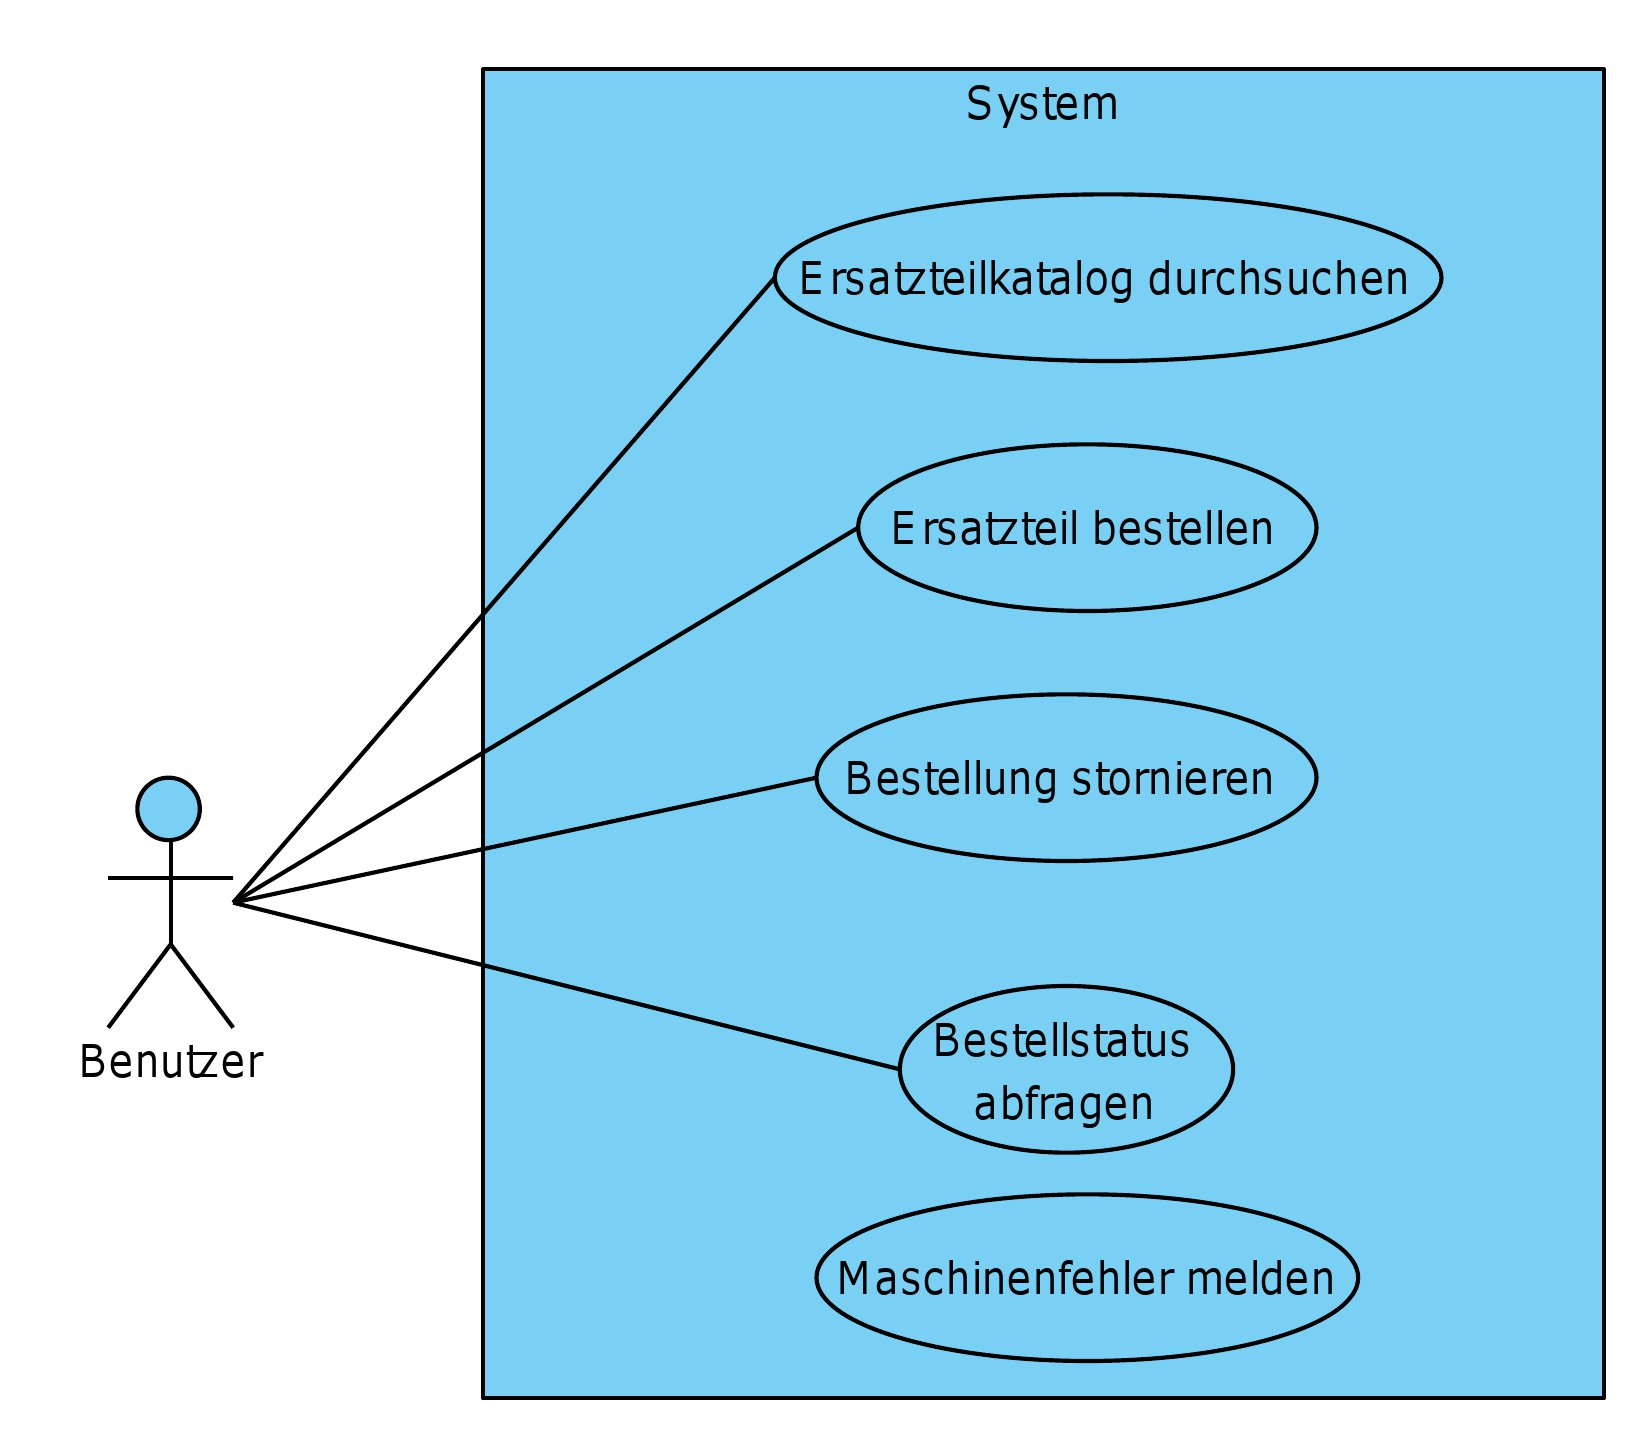
\includegraphics[width=0.8\textwidth]{Ersatzteilkatalog_use_case}
		      \caption{Gesch�ftsanwendungsf�lle Use-Case-Diagramm}
		      \label{fig:usecase}
		\end{figure}


		\begin{itemize}
            \item Ersatzteilkatalog durchsuchen / Benutzer
            \item Ersatzteil bestellen / Benutzer
            \item Bestellung stornieren / Benutzer
            \item Bestellstatus abfragen / Benutzer
            \item Maschinenfehler melden / System
          \end{itemize}
      	
      	
      	\begin{itemize}
            \item Die Transformationen erzeugen dabei aus den Elementen des
            Quellmodells die Elemente des Zielmodells. �blicherweise laufen
            die Transformationen von der abstrakteren zur konkreteren Schicht
            (CIM -> PIM -> PSM -> Code)
            \item Ist hier wirklich eine komplette Transformation n�tig? Dann
            m�ssen mit OAW komplett alle Cartridges erstellt werden
            \item Ansonsten Acceleo f�r Model-zu-Code Transformation; Daf�r
            muss nur 1 Template je umzusetzendes Betriebssystem geschrieben
            werden und die Templates k�nnen aus vorhandenem Beispielcode
            generiert werden (sehr schnelle Erstellung von Templates m�glich)
            %\item Evtl. AndroMDA (wird allerdings seit 2006 nicht mehr
            %weiterentwickelt...)
            \item Kommerzielle L�sungen?
          \end{itemize}
          
          
          \subsection{Vorhandene Modellierungs-/Transformationstools auf dem
          Markt}
          
          \subsubsection{OAW}
          \subsubsection{Acceleo}
          \subsection{Wahl der zu benutzenden Tools}
          
          Visual Paradigm
          
          
